\chapter{Theoretische Grundlagen}\label{sec:basics}

In diesem Kapitel werden die für den Forschungshintergrund und die Entwicklung des Prototyps wichtigen theoretischen Grundlagen beschrieben.
Zunächst werden verschiedene Theorien zu Kommunikationsmodellen und kooperativer Kommunikation vorgestellt, die dem Modell dieser Anwendung zugrunde liegen.
Im Anschluss daran werden die in der Ludologie beschriebenen Akteurstypen vorgestellt, die sich in den Teilnehmenden dieser Masterarbeitsstudie widerspiegeln.
Allgemein ist bekannt, dass Video- und Computerspiele drei verschiedene Modi haben können: Singleplayer, Multiplayer und Mischformen. Da im Rahmen dieser Studie ein Multiplayer-Spiel konzipiert und umgesetzt wurde, werden im weiteren Verlauf verschiedene Kategorien von Multiplayer-Spielen vorgestellt. Außerdem werden die damit einhergehenden Netzwerkinfrastrukturen dargestellt, die für die aktuelle sowie eine potenzielle zukünftige Entwicklung relevant sind. Zum Schluss erfolgt ein Einblick in die \ac{AR}. [Es fehlt noch die definitopn von adventure games]!!!!!!!!!!

\section{Kommunikationsforschung}

Die Kommunikationsforschung umfasst innerhalb der Kommunikationswissenschaft viele Gebiete. Aus diesem Grund muss zunächst der Begriff \say{Kommunikation} definiert werden.

Kommunikation bezeichnet den Prozess des Sendens und Empfangens von Botschaften, den Austausch von Informationen sowie die Interaktion mit anderen. Sei es im persönlichen Kontakt oder über eine Vielzahl etablierter und neuer Technologien (vgl. \citealp[S. 18]{krcmar_communication_2016}).
Bentele und Beck präzisieren diese Definitionindem sie ergänzen, dass die wechselseitige Bedeutungsübermittlung sowohl sprachlich-symbolisch als auch nonverbal erfolgen kann, etwa durch Blicke oder Gesten (vgl. \citealp[S. 20]{bentele_information_1994}).

\begin{quote}
\textit{\enquote{Kommunikation wird somit als soziale Interaktion zwischen zwei oder mehreren Menschen verstanden, die dem Austausch von Informationen, Gedanken, Erfahrungen etc. innerhalb einer aktuellen Situation dient.}} \cite[S. 19]{becker_praxishandbuch_2018}
\end{quote}

Sobald Menschen miteinander kommunizieren, geschieht dies in der Regel auf mehreren Ebenen gleichzeitig. Dabei wird zwischen verbaler, paraverbaler und nonverbaler Kommunikation unterschieden. 

Verbale Informationen können gelesen ebenfalls einen Sinn ergeben.
Nonverbale Informationen durch Mimik, Gestik und die Körpersprache können nur dann verstanden werden, wenn der Gegenüber sie sieht. 
Paraverbale Informationen werden durch die Betonung, Stimmlage, Pausenlängen etc. übermittelt. Sie können nur durch das Hören gedeutet werden (vgl. \citealp[S. 33]{ebert_formen_2018}).

Kommunikation ist durch gegenseitige Abhängigkeiten geprägt: Während der Sender das Geschehen aktiv gestaltet, nimmt der Empfänger Informationen auf und interpretiert sie. Dabei ist nicht jede Kommunikation bewusst beabsichtigt. Die Abgrenzung zwischen Kommunikation und Interaktion ist schwierig, da Kommunikation häufig als Bestandteil von Interaktion verstanden wird. Kommunikatives Verhalten wird sowohl durch bewusste Erfahrungen und Lernprozesse als auch durch unbewusste Verhaltensmuster beeinflusst (vgl. \citealp[S. 20]{becker_praxishandbuch_2018}.

Um besser zu verstehen, welche Prozesse innerhalb der Kommunikation ablaufen und wie sie erlebt und interpretiert wird, wurden im Laufe der Zeit zahlreiche Theorien und Modelle entwickelt (vgl. \citealp[S. 311]{schwarz_grundlagen_2019}).

Diese \say{Kommunikationsmodelle} berücksichtigen insbesondere den sozialen Kontext. Sie sind keine exakten Abbilder kommunikativer Realität, sondern vereinfachte Darstellungen realer Erscheinungsformen und Prozesse (vgl. \citealp[S. 56]{maletzke_kommunikationswissenschaft_1998}).

\subsection{Kommunikationsmodell nach Shannon und Weaver}

\begin{figure}[ht]
\centering
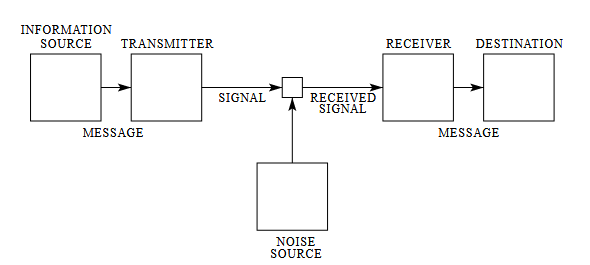
\includegraphics[width=1\linewidth]{content/pictures/shannon-weaver.PNG}
\caption{Kommunikationsmodell von Shannon und Weaver (Quelle: \citealp[S. 2]{shannon_mathematical_1948})}
\label{fig:shannon-weaver-modell}
\end{figure}

Abbildung \ref{fig:shannon-weaver-modell} zeigt das wohl bekannteste Klassifikationsmodell von Shannon und Weaver. Es beschreibt jedoch keine soziale Kommunikation, sondern einen technischen Signaltransfer zwischen Sender und Empfänger. Im Fokus steht die physikalische Informationsübertragung, beispielhaft in der Form eines Telefongesprächs (vgl. \citealp[S. 92]{scheufele_kommunikationstheorien_2004}). 

Dabei geht das Modell von einer Informationsquelle aus, die eine Nachricht an ein Ziel übermitteln möchte. Die Nachricht wird zunächst von einem Transmitter in ein analoges Signal umgewandelt und anschließend an ein Empfangsgerät gesendet. Während der Übertragung kann es zu Störungen kommen, durch externe Geräusche oder technische Einflüsse, die das Signal verfälschen. Diese Störsignale werden gemeinsam mit der ursprünglichen Nachricht übermittelt. Am Ende des Prozesses empfängt das Empfangsgerät die Nachricht, sodass der Empfämger die Nachricht, einschließlich möglicher Störungen, bspw. als Audiosignal wahrnehmen kann.

\subsection{Kommunikationsmodell nach Osgood und Schramm}
Während das Modell von Shannon und Weaver die technischen Aspekte der Informationsübertragung in den Mittelpunkt stellt, stößt es bei der Beschreibung sozialer Kommunikation an seine Grenzen. Insbesondere der interaktive und dynamische Charakter zwischenmenschlicher Verständigung bleibt unberücksichtigt.

\begin{figure}[ht]
\centering
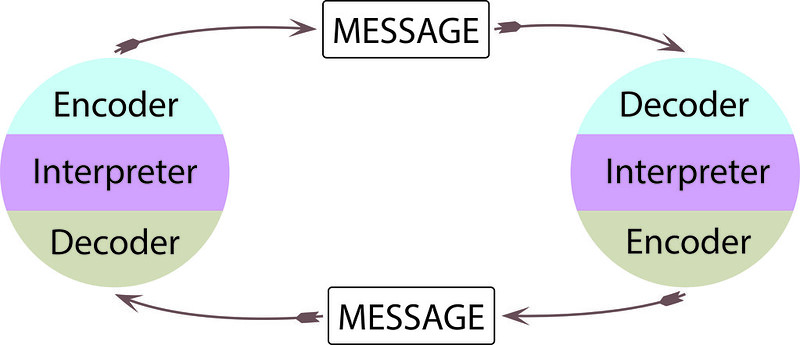
\includegraphics[width=1\linewidth]{content/pictures/osgood-schramm.jpg}
\caption{Kommunikationsmodell von Osgood und Schramm (Quelle: \citealp{wrench_24_2021})}
\label{fig:osgood-schramm-modell}
\end{figure}

Das in Abbildung \ref{fig:osgood-schramm-modell} gezeigte Modell unterscheidet sich grundlegend von früheren linearen Modellen wie dem von Shannon und Weaver. Es betont stattdessen die wechselseitige Struktur und Zirkularität von Kommunikation. Kommunikation ist hier kein einmaliger Signaltransfer, sondern ein kontinuierlicher Prozess, bei dem beide Gesprächspartner die Bedeutung einer Botschaft gemeinsam aushandeln. Feedback ist dabei kein optionales, sondern ein zentrales Element. Es ermöglicht Missverständnisse zu klären, Reaktionen einzuholen und Aussagen zu präzisieren (vgl. \citealp{noauthor_osgood_2024}). 

Das Besondere an dem Modell ist, dass persönliche Merkmale der Kommunikationsteilnehmer, wie individuelle Erfahrungen, kulturelle Prägungen, Bildungshintergründe und Erwartungen in den Gesprächszyklus einfließen. Auf Grundlage dieser Faktoren erfolgt ein Codoierungs- und Decodierungsprozess in sprachliche und nicht-sprachliche Zeichen, die vom Empfänger interpretiert werden (vgl. \citealp{noauthor_osgood_2024}). 

\subsection{Kommunikationsmodell nach Badura}
Als Erweiterung des Modells von Osgood und Schramm kann das Modell von Badura gesehen werden (vgl. Abbildung \ref{fig:badura-modell}).

\begin{figure}[ht]
\centering
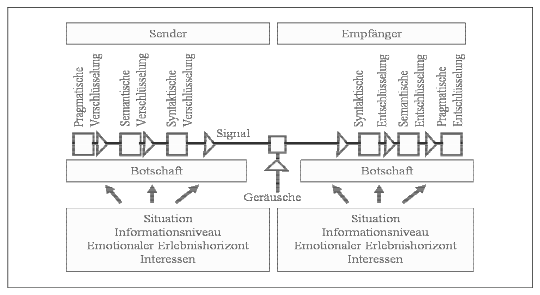
\includegraphics[width=1\linewidth]{content/pictures/badura.PNG}
\caption{Kommunikationsmodell von Badura (Quelle: \cite{badura_kommunikation_1992}, \cite[S. 93]{scheufele_kommunikation_2007})}
\label{fig:badura-modell}
\end{figure}

Das Kommunikationsmodell unterscheidet zwischen semantischen, syntaktischen und pragmatischen Aspekten der Sprache bzw. kommunikativen Botschaften. Der Rahmen in dem Kommunikation stattfindet, umfasst in diesem Modell vier zentrale Aspekte der Kommunikationssituation: das Informationsniveau der Teilnehmer, ihrem emotionalen Erlebnishorizont in den jeweiligen Situationen sowie ihre Interessen und Ziele (vgl. \citealp[S. 93]{scheufele_kommunikation_2007}).

\subsection{Das Kommunikationsquadrat nach Schultz von Thun}
Während die zuvor genannten Modelle den Ablauf und die Zirkularität von Kommunikation beschreiben, rückt das Kommunikationsquadrat die inhaltliche Vielschichtigkeit jeder Botschaft in den Mittelpunkt.

\begin{figure}[ht]
\centering
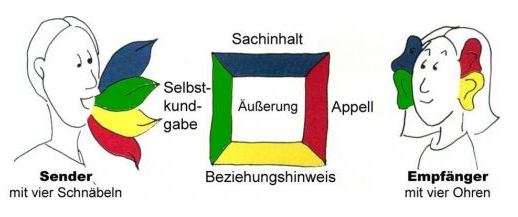
\includegraphics[width=1\linewidth]{content/pictures/Kommunikationsquadrat.PNG}
\caption{4 - Ohren Modell von Schulz von Thun (Quelle: \citealp{noauthor_kommunikationsquadrat_nodate})}
\label{fig:four-ears}
\end{figure}

Das in Abbildung \ref{fig:four-ears} gezeigte Modell, auch \say{Nachrichtenquadrat} oder \say{Kommunikationsquadrat} genannt, zeigt, dass jede Nachricht vier Botschaften gleichzeitig übermittelt. Diese sind die Sachinformation, die darüber Auskunft gibt, worum es inhaltlich geht. Die Selbstkundgabe, bei der der Sender Informationen über sich selbst preisgibt. Dem Beziehungshinweise, der erkennen lässt, in welchem Verhältnis der Sender zum Empfänger steht. Sowie der Appell durch den der Sender versucht, beim Empfänger eine bestimmte Reaktion oder Handlung auszulösen (vgl. \citealp{noauthor_kommunikationsquadrat_nodate}).

Die gewählten Äußerungen entstammen dabei aus den sog. \say{vier Schnäbeln} des Senders, die auf die \say{vier Ohren} des Empfängers treffen (vgl. \citealp{noauthor_kommunikationsquadrat_nodate}). Schulz von Thun geht dabei davon aus, dass jede Nachricht mit vier Ohren empfangen wird (vgl \citealp[S. 23]{becker_praxishandbuch_2018}). 

Das Modell ist im Kern ein Ausdrucksmodell der Kommunikation. Es soll einerseits dabei helfen, die Ursachen möglicher Missverständnisse besser zu verstehen. Andererseits wird jedoch kritisiert, dass es sowohl den Charakter der Kommunikation als gemeinschaftliche Handlung, als auch den steuernden Aspekt des Sprechens vernachlässigt (vgl \citealp[S. 23]{becker_praxishandbuch_2018}). Es berücksichtigt somit nicht die Möglichkeit des Nachfragens beim Sender. Stattdessen legt das Modell nahe, dass jeder Äußerung ein einziger \say{wahrer} Bedeutungskern innewohne (vgl \citealp[S. 23]{becker_praxishandbuch_2018}). 

\subsection{Konversationsmaximen von Grice}
Grice erweitert die o. g. Theorien insofern, das Kommunikation nicht nur über das Gesagte, sondern auch über das Implizierte funktioniert (vgl. \citealp[S. 43f]{grice1975logic}). 

Ausgangspunkt seiner Überlegungen sind die Bedingungen, unter deren Konversationen stattfinden. In der Regel bestehen sie nicht aus zufälligen und unzusammenhängenden Äußerungen, sondern folgen einer bestimmten Struktur. Daraus leitet Grice das sogenannte Kooperationsprinzip ab. Dieses besagt, dass ein Gesprächsbeitrag so gestaltet sein soll, wie es der Zweck oder die Richtung des Gesprächs im jeweiligen Stadium erfordert (vgl. \citealp[S. 45]{grice1975logic}).

Aus diesem Prinzip ergeben sich vier Maximen der Kommunikation. 

Die Maxime der Quantität (Informationsmenge) besagt, dass der gesprochene Beitrag so informativ wie erforderlich, jedoch nicht informativer als nötig gestaltet sein soll. Die Maxime der Qualität (Wahrheit) betrifft die Aufrichtigkeit der Nachricht. Es soll nichts gesagt werden, was der Sprecher für falsch hält oder wofür keine ausreichenden Belege vorliegen. Die Maxime der Relevanz fordert, dass der Beitrag sachbezogen und zum Gesprächsziel passend ist. Schließlich umfasst die Maxime der Modalität (Art und Weise des Gesagten) die Vermeidung von Unklarheiten und Mehrdeutigkeiten sowie das Vermeiden von Ausschweifungen und die Forderung nach Ordnung in der Darstellung (vgl. \citealp[S. 45f]{grice1975logic}).

Wird gegen eine der Maximen verstoßen, kann der Gesprächspartner davon ausgehen, dass dies nicht zufällig, sondern absichtlich geschieht. Somit wird eine zusätzliche Bedeutung impliziert. In solchen Fällen entsteht eine implizite Bedeutung, die über das wörtlich Gesagte hinausgeht. Doe Maximen dienen somit als Interpretationshilfe, um solche kommunikativen Hinweise richtig zu deuten (vgl. \citealp[S. 49f]{grice1975logic}).

\subsection{Axiome der Kommunikationen nach Watzlawik et. al}
Ergänzend zu den davor dargestellten Modellen betrachten Watzlawik, Beavin und Jackson zwischenmenschliche Kommunikation aus einer systematisch-konstruktivistischen Perspektive. Im Mittelpunkt steht dabei Kommunikation als wechselseitiges Verhalten innerhalb sozialer Kontexte (vgl. \citealp{Watzlawick2016-km}). 

Zur Beschreibung dieses Verständnisses definieren die Autoren fünf Grundprinzipien (Axiome) mit denen sich menschliche Kommunikation systematisch erklären lässt (vgl. \citealp{Watzlawick2016-km}):
\begin{itemize}
    \item \say{Man kann nicht nicht kommunizieren}, da jedes Verhalten kommunikativen Charakter besitzt, ist Kommunikation unausweichlich (vgl. \citealp[S. 53]{Watzlawick2016-km}).
    \item \say{Jede Kommunikation hat einen Inhalts- und einen Beziehungsaspekt, derart, dass letzterer den ersteren bestimmt und daher eine Metakommunikation ist.} \cite[S. 64]{Watzlawick2016-km}
    \item \say{Die Natur einer Beziehung ist durch die Interpunktion der Kommunikationsabläufe seitens der Partner bedingt.} Die Kommunikation verläuft zirkular. (vgl. \citealp[S. 69]{Watzlawick2016-km})
    \item Menschliche Kommunikation nutzt sowohl digitale als auch analoge Ausdrucksformen. Digitale Kommunikation ist logisch strukturiert, aber in Beziehungssituationen bedeutungsarm. Analoge Kommunikation hingegen transportiert Beziehungsinhalte wirkungsvoll, ist jedoch weniger eindeutig in der Bedeutung (vgl. \citealp[S. 77]{Watzlawick2016-km}).
    \item \say{Zwischenmenschliche Kommunikationsabläufe sind entweder symmetrisch oder komplementär, je nachdem, ob die Beziehung zwischen den Partnern auf Gleichheit oder Ungleichheit beruht} \cite[S. 80]{Watzlawick2016-km}
\end{itemize}

\subsection{Gelingende Kommunikation nach Carl Rogers}
Dieses Modell geht einen Schritt weiter, als die zuvor behandelten Modelle. Es untersucht, wie Kommunikation zwischen den Teilnehmenden erfolgreich gelingen kann.

Rogers identifiziert drei zentrale Prinzipien, die gelingende Kommunikation ausmachen: Echtheit (Kongruenz), Empathie und Wertschätzung (bedingungslose Akzeptanz) (vgl. \citealp{jesse_carl_2025}).

Die Echtzeit beschreibt die Offenheit der Gesprächspartner und die Vermeidung von künstlichem Verhalten. Dadurch soll ein Gefühl von Sicherheit und Vertrauen entstehen. 

Die Empathie meint das Einfühlen in die Lage des Gegenübers, um dessen Gefühle und Gedanken aus dessen Perspektive zu verstehen. Dieses Verständnis fördert eine tiefere emotionale Verbindung zwischen den Gesprächspartnern.

Die Wertschätzung umfasst das uneingeschränkte Akzeptieren und Wertschätzen der anderen Person, unabhängig von deren Verhalten oder Meinung. Aus dieser Wertschätzung heraus sollen sich die Beteiligten sicher und geschützt fühlen.

\section{Spielertypen}
Die kommunikationswissenschaftlichen Aspekte bilden zwar den Schwerpunkt dieser Arbeit, doch wurden auch ludologische Gesichtspunkte
berücksichtigt. Dabei handelt es sich um die wissenschaftliche Auseinandersetzung mit dem Spielen selbst (vgl. \citealp{institut_fur_ludologie_spielforschung_nodate}). 

Im Hinblick auf die Konzeption und Entwicklung eines Spiels ist es wichtig, die Eigenschaften des Spielsystems so zu gestalten, dass sie Begeisterung und Engagement bei der gewünschten Zielgruppe hervorrufen. Deshalb muss zunächst die Zielgruppe in verschiedene Typen eingeteilt werden. Die Ludologie unterscheidet hierfür verschiedene Spielertypen. Zwar ist nicht jeder Mensch ein eindeutiger \say{Spielertyp}, dennoch lassen sich unterschiedliche Spielertypen grundsätzlich über spezifische Spielelemente ansprechen (vgl. \citealp{institut_fur_ludologie_spielertypen_nodate}).

\subsection{Nach Bartle}
1996 beschäftigte sich Richard Bartle mit der Frage, welche Spielertypen in der Ludologie unterschieden werden können. Dabei ging es zunächst um Klassifizierungen von Ansätzen, die beim Spielen von sogenannten \ac{MUD}s existieren (vgl. \cite{bartle_hearts_1996}). Diese Klassifizierungen werden noch heute für die Einteilung in Spielertypen herangezogen.

Bartle unterscheidet bei der Einteilung der Spielertypen zwei grundlegende Interessen (vgl. Abbildung \ref{fig:bartle-muds}):

\begin{figure}[ht]
\centering
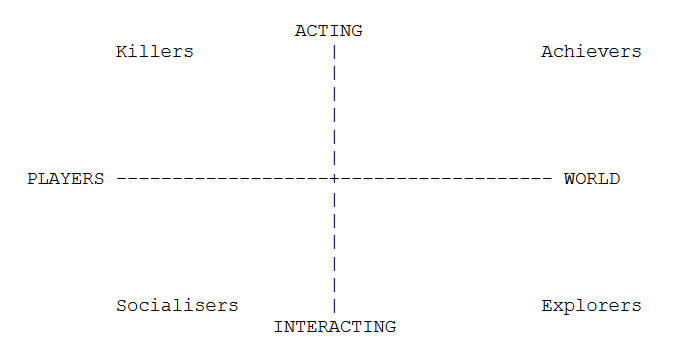
\includegraphics[width=1\linewidth]{content/pictures/basic_interests.PNG}
\caption{Interessen Graph nach Bartle (Quelle: \citealp{bartle_hearts_1996})}
\label{fig:bartle-muds}
\end{figure}

Auf der X-Achse wird unterschieden, ob Spieler ihre Spielerfahrung über das Verhalten der anderen Mitspieler (Players) oder über die Spielwelt (World) definieren. Entlang der Y-Achse wird unterschieden, ob Spieler eher selbst aktiv Einfluss auf die Spielwelt nehmen möchten (Acting) oder ob sie eine tiefere Interaktion mit ihr eingehen wollen (Interacting).

Die daraus resultierenden Typen sind (vgl. \citealp{bartle_hearts_1996}):
\paragraph{Achiever}
Sie sind daran interessiert, auf die Spielwelt einzuwirken und alle ihnen gestellten Aufgaben mit Erfolg zu absolvieren. Ihr Status im Spiel ist ihnen wichtig - ebenso wie die Effizienz, mit der sie Fortschritte erzielen.

\paragraph{Explorer}
Sie wollen vom Spiel überrascht werden und intensiv mit der Spielwelt interagieren. Die virtuelle Welt löst ein Gefühl des Staunens aus, nach dem sie aktiv suchen. Sie sind stolz auf das Wissen, das sie im Spiel sammeln. Das erlangte Wissen möchten sie gerne an neue Spieler weitergeben.

\paragraph{Socialiser}
Sie wollen mit anderen Spielern interagieren, meist über Gespräche, aber auch durch ungewöhnliche oder kreative Verhaltensweisen. Andere Menschen kennenzulernen und mehr über sie zu erfahren, ist für sie wertvoller als für andere. Die Spielwelt dient dabei lediglich als Kulisse - entscheidend sind für sie die Begegnungen mit anderen Charaktere. Sie sind stolz auf Freundschaften, ihre Kontakte und ihren Einfluss.

\paragraph{Killer}
Sie sind daran interessiert, auf andere Spiele einzuwirken und mit ihnen zu interagieren - häufig ohne deren Einverständnis. Sie wollen ihre Überlegenheit gegenüber anderen Menschen demonstrieren und sind stolz auf ihren Ruf, sowie auf ihre oft geübten Kampffähigkeiten.

\subsection{Erweiterte Einteilungen}
Bartle ist nicht der Einzige, der sich mit Spielertypen auseinandergesetzt hat. Seine Forschung bildet jedoch ein grundlegendes Fundament, das in der weiteren wissenschaftlichen Auseinandersetzung intensive Diskussionen innerhalb der Forschungs- und Game-Design-Community ausgelöst hat. Im folgenden werden weitere Typisierungen und Einteilungen vorgestellt.
\begin{quote}
    \textit{
        \enquote{Player types are not a defined concept and any categorization of players or users needs to occur within the context of a particular application or domain. Play-personas are suggested as a useful tool that can be used to put player type research into practice as part of the design process of gamified systems.}
    } 
    \cite{dixon_player_nodate}
\end{quote}

\paragraph{Dixon} 
stellt Spieler-Personae ????? ist das Wort richtig?  vor, die analog zum \ac{UCD}-Prozess eingesetzt werden können. Dadurch muss im Designprozess nicht strikt zwischen Motivation, Verhalten und Vorlieben unterschieden werden, da die Personae als ausführliche, erzählerische Darstellung gedacht sind (vgl. \citealp{dixon_player_nodate}).

\paragraph{Bateman und Boon}
entwickelten in ihrer 2005 erschienenen Studie zur Bestimmung des ersten Modells des Demographic Game Design (DGD1) vier Spielstile, die sie durch die Einbeziehung des \ac{MBTI} ableiteten (vgl. \citealp{noauthor_mbti_nodate, bateman_21st_2005}).
Die vier Spielstile lauteten: Conquerer (Eroberer), Manager (Manager) Wanderer (Wanderer) und Participant (Teilnehmer).

In einer zweiten Studie wurden vier hypothetische Spielstile entwickelt, die auf einer Untersuchung von \cite{berens_understanding_2000} basierten (vgl. \citealp{bateman_player_2012}). Die daraus resultierenden Stile lauteten: Logistical, Tactical, Strategic und Diplomatic.

Im Kern sind diese Modelle Weiterentwicklungen bzw. Ableitungen von Bartles ursprünglicher Typologie (vgl. \citealp{institut_fur_ludologie_spielertypen_nodate}).

\paragraph{Yee}
Nick Yee entwickelte ein empirisch fundiertes Modell zur Beschreibung von Spielmotivationen in Online-Spielen, das bis heute einen bedeutenden Einfluss auf die Ludologie hat. Anhand eines faktorenanalytischen Ansatzes untersuchte er eine Vielzahl an Daten aus Online-Umfragen und identifizierte dabei zehn spezifische Motivationsgruppen, die sich in drei übergeordnete Hauptkategorien einordnen lassen (vgl. Abbildung \ref{fig:nick_yee_motivations}):

\begin{figure}[ht]
\centering
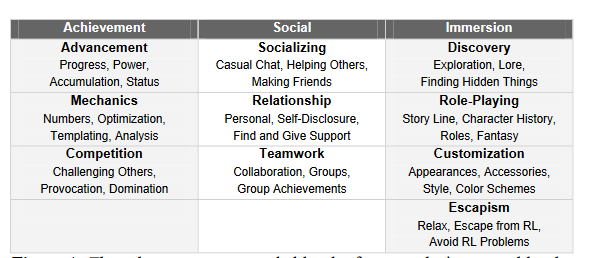
\includegraphics[width=1\linewidth]{content/pictures/nick_yee_categorizations.PNG}
\caption{Motivationsgruppen nach Nick Yee (Quelle: \citealp[S. 5]{yee_motivations_2006})}
\label{fig:nick_yee_motivations}
\end{figure}

Die Achievement-Komponente umfasst den Fortschritt im Spiel, sowie das damit einhergehende Verlangen Macht zu erlangen, schnell voranzukommen und Symbole für Reichtum oder Status zu erwerben. Zudem besteht ein Interesse daran, die Spielmechanik zu analysieren, die Regeln und Systeme zu verstehen, um die Leistung der Spielfigur zu optimieren. Auch spielt der Wettbewerb eine zentrale Rolle. Esbesteht der Wunsch, sich mit anderen zu messen und gegen sie anzutreten (vgl. \citealp[S. 5]{yee_motivations_2006}).

Die soziale Komponente beschreibt das Bedürfnis nach Sozialisierung. Spieler haben Interesse daran, anderen zu helfen und sich mit ihnen zu unterhalten. Daraus entstehen Beziehungen, bei denen der Wunsch besteht, langfristige und bedeutungsvolle Bindungen zu anderen aufzubauen. Teamarbeit ist dabei gewünscht, um gemeinsame Ziele zu erreichen oder sich im Wettbewerb zu behaupten (vgl. \citealp[S. 6]{yee_motivations_2006}).

Die Immersion-Komponente beschreibt das Entdecken der Spielwelt und das damit verbundene Finden von Objekten, sowie das Erlangen von Wissen, das den meisten anderen Spielern unbekannt ist. Rollenspiel-Elemente sind besonders wichtig, um den Spielfiguren Hintergrundgeschichten zu geben und gemeinsam improvisierte Erzählungen zu entwickeln. Der Spielavatar sollte zudem anpassbar sein, damit persönliche Vorlieben und der individueller Stil der Spieler zum Ausdruck kommen kann. Die Spielwelt dient auch als Mittel um dem Alltag zu entfliehen und den Problemen der realen Welt zu entkommen (vgl. \citealp[S. 6]{yee_motivations_2006}).

\paragraph{weitere Modelle}
Im Zuge der fortschreitenden Forschungen entstanden weitere Modelle wie zum Beispiel das Gamer Motivation Model, das auf Basis der Forschung von Nick Yee entwickelt wurde (vgl. \citealp{institut_fur_ludologie_spielertypen_nodate}):

\begin{figure}[ht]
\centering
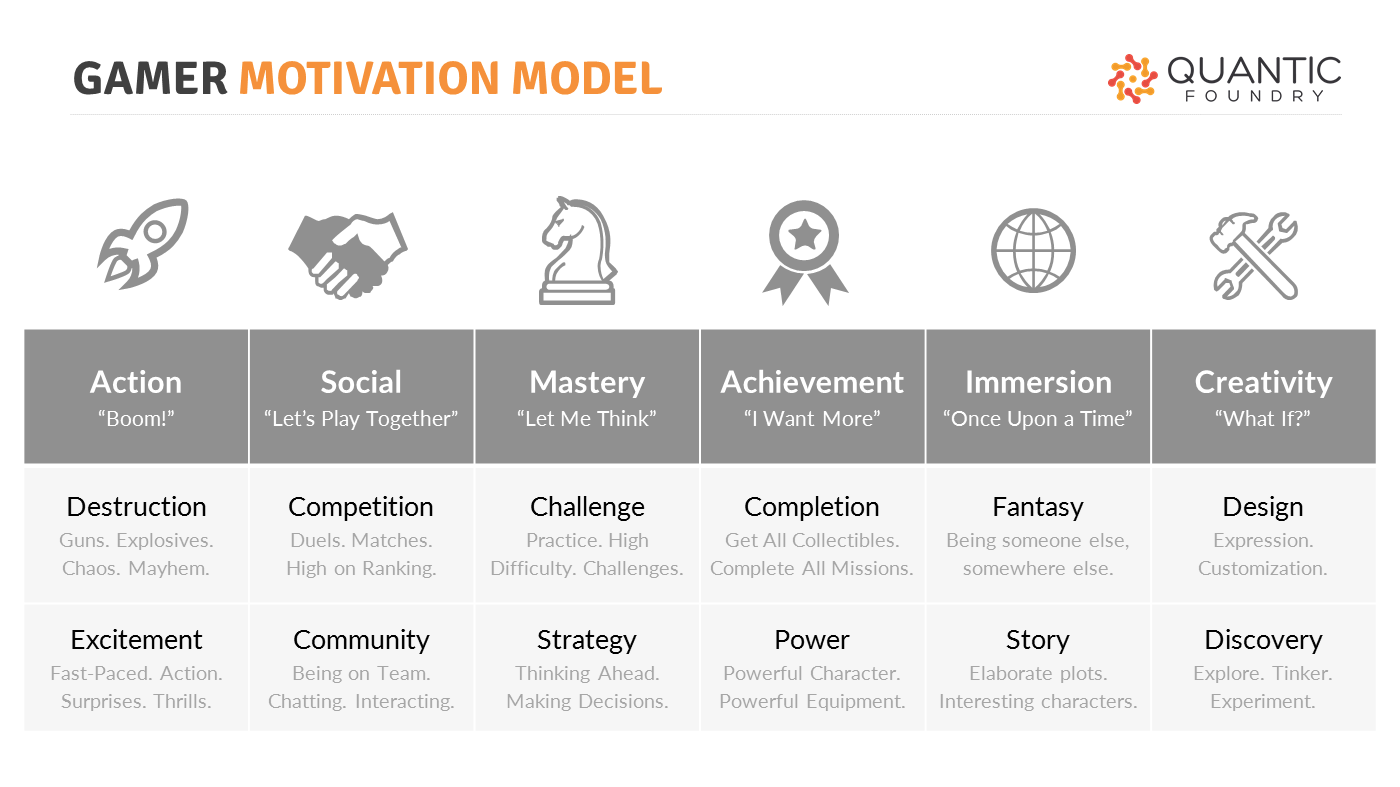
\includegraphics[width=1\linewidth]{content/pictures/gamer_motivations_model.png}
\caption{Gamer Motivation Model der QUANTIC FOUNDRY (Quelle: \citealp{noauthor_quantic_nodate})}
\label{fig:gamer_motivation_model}
\end{figure}

Ein weiteres Modell, das in der Arbeit von Bateman genannt wird, ist das BRAINHEX-Model, bei dem die verschiedenen Spielertypen in hexagonaler Anordnung platziert sind (vgl. Abbildung: \ref{fig:brain-hex}):

\begin{figure}[ht]
\centering
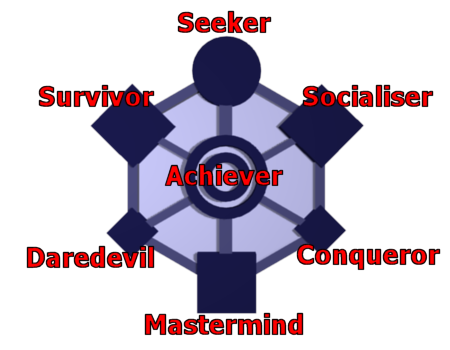
\includegraphics[width=1\linewidth]{content/pictures/brainhex-classes.png}
\caption{Brainhex-Model Darstellung von \citealp{noauthor_i_nodate} nach \citealp{nacke_brainhex_2013}}
\label{fig:brain-hex}
\end{figure}

\section{Multiplayer-Spiele}
Im Vergleich zu Einzelspieler-Spielen existieren bei Multiplayer-Spielen nicht nur Unterschiede im Genre, sondern auch in den Spielrollen (Symmetrie / Asymmetrie) sowie in den Spielzeitpunkten, zu denen die Spielteilnehmer an ihrem Spielfortschritt weiterarbeiten (Synchron / Asynchron). Auf dem Spielemarkt existieren außerdem Multiplayer-Spiele, die unterschiedliche Medientechniken verwenden. Teilweise dienen diese Medientechniken dazu, Cross-Plattform Funktionalität zu gewährleisten (vgl. \citealp{larian_studios_baldurs_2023}), oder sie sind integraler Bestandteil des Gamedesigns (vgl. \citealp{steel_crate_games_keep_2015}).

Da im Kontext von \say{Connecting-Minds} die Spieler zeitgleich in einer Sitzung gemeinsam spielen, wird im Folgenden auf die Symmetrie und Asymmetrie von Computer- und Videospielen eingegangen.

\subsection{Symmetrische Multiplayer}
Symmetrische Spiele sind solche, bei denen alle Spieler die gleichen Spielregeln haben und das gleiche Spielziel verfolgen. Viele traditionelle Spiele wie Schach sowie Computer- und Videospiele wie \say{Mario Kart} oder \say{Minecraft} (vgl. \citealp{nintendo_mario_1992, mojang_willkommen_2009}) sind symmetrische Multiplayer-Spiele, bei denen für jeden Spieler das gleiche Ziel gilt (vgl. \citealp[S. 12]{adams_fundamentals_2013}).

\subsection{Asymmetrische Multiplayer}
Asymmetrische Spiele hingegen können unterschiedlichen Spielern unterschiedliche Regeln zugestehen und ggf. verfolgen die Spieler unterschiedliche Ziele (vgl. \citealp[S. 12]{adams_fundamentals_2013}). Sie sind sowohl in kooperativen als auch kompetitiven Spielen weit verbreitet und werden bspw. in Form verschiedener \say{Helden} oder \say{Klassen} umgesetzt. So gibt es z.B. in \say{Overwatch} oder \say{League of Legends} (vgl. \citealp{noauthor_league_2025, noauthor_overwatch_nodate}) unterschiedliche \say{Support}-Charaktere, deren Aufgabe es ist, das Team zu heilen (vgl. \citealp[S. 307f]{smilovitch_birdquestvr_2019}).
Außerdem ermöglichen asymmetrische Spiele, dass Spieler mit unterschiedlichen Fähigkeiten und Fähigkeitsniveaus gemeinsam spielen können. Ein asymmetrisches Design kann zudem die Inklusivität in Spielen fördern (vgl. \citealp[S. 308]{smilovitch_birdquestvr_2019}).

\subsection{Hybride Multiplayer}\label{sec:hybrid-multiplayer}
Wie Lotz in ihrer Bachelor-Arbeit beschrieben hat, unterscheiden sich Multiplayer auch in der verwendeten Medientechnik (vgl. \citealp[S. 6f]{lotz_konzeption_2021}). Es gibt sogenannte hybride Spiele wie \say{New Super Mario Bros U} (vgl. \citealp{nintendo_mario_2012}).

\begin{figure}[ht]
\centering
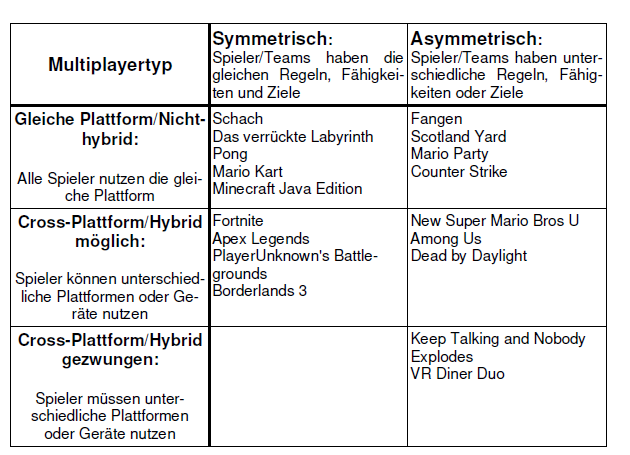
\includegraphics[width=1\linewidth]{content/pictures/lotz_hybrid_multiplayer.PNG}
\caption{Unterscheidung Multiplayertypen (Quelle: \citealp[S.6]{lotz_konzeption_2021})}
\label{fig:lotz_multiplayer_types}
\end{figure}

Wie Abbildung \ref{fig:lotz_multiplayer_types} zeigt, können Multiplayer-Spiele hinsichtlich ihrer Medientechnik in drei Kategorien eingeteilt werden.
Spiele wie \say{Mario Kart} oder \say{Minecraft} können nur auf der gleiche Plattform gespielt werden. Bei Spielen wie \say{Among Us} oder \say{Fortnite} ist die Plattform, auf der gespielt wird, nicht relevant, da eine Cross-Play-Funktionalität gegeben ist. Jeder kann auf der Plattform mitspielen, die er besitzt. Die dritte Kategorie umfasst Spiele, bei denen die Spieler gezwungen werden, unterschiedliche Plattformen zu nutzen. In \say{Keep talking and nobody explodes} ist dies der Kern des Gamedesigns.

\section{Spielweisen von Multiplayer-Spielen}
Nachdem die unterschiedlichen Strukturen und technischen Formen von Multiplayer-Spielen behandelt wurden, ist es nun wichtig, die verschiedenen Spielweisen zu betrachten. Multiplayer-Spiele können dabei in kompetitive, kollaborative und kooperative Spiele unterteilt werden (vgl. \citealp[S. 25f]{zagal_collaborative_2006}).

\subsection{Kompetitiv}
Kompetitive Spiele sind solche, bei denen Spieler oder Teams gegeneinander antreten, um ein bestimmtes Ziel zu erreichen, wobei der Erfolg des einen oft den Misserfolg des anderen bedeutet. In diesen Spielen ist das Spiel selbst neutral und agiert nicht aktiv im Wettbewerb (vgl. \citealp{noauthor_game_2014}; \citealp[S. 25]{zagal_collaborative_2006}).

\subsection{Kollaborativ}
Kollaborative Spiele sind solche, bei denen alle Spieler - ähnlich wie in Kooperationsspielen - gemeinsam gegen das Spiel verlieren können. Allerdings können sie nicht gemeinsam gewinnen. Diese Spiele sind im Kern meist kompetitiv, beinhalten jedoch die Möglichkeit einer kollektiven Niederlage. Die Spieler müssen zu einem gewissen Maß zusammenarbeiten, um nicht zu verlieren (vgl. \citealp{noauthor_game_2014};  \citealp[S. 25]{zagal_collaborative_2006}).

\subsection{Kooperativ}
Bei Kooperationsspielen ist es möglich, dass alle Spieler gemeinsam gegen das Spiel verlieren oder gemeinsam gewinnen können. Ein Sieg wird erreicht, wenn das Spiel gemeinsam \say{besiegt} wird oder dadurch, dass ein festgelegtes Ziel kollektiv oder individuell erreicht werden kann (vgl. \citealp{noauthor_game_2014}; \citealp[S. 25]{zagal_collaborative_2006}).

\section{Netzwerkinfrastrukturen}\label{sec:basics-network-structures}
Um ein plattformunabhängiges Multiplayer-Spiel entwickeln zu können, muss zunächst geklärt werden, wie die Netzwerkinfrastruktur der Anwendung aufgebaut sein soll. Es existieren zahlreiche Ansätze, die jeweils für verschiedene Anwendungszwecke konzipiert sind. Diese werden im Folgenden vorgestellt.

\subsection{Distributed Authority}
Bei einer \say{Distributed Authority}-Netzwerktopologie übernimmt jeder im Netzwerk verbundene Spielclient gemeinsam jeweils die Verantwortung für das Erstellen und Verwalten von Objekten im Netzwerk. Jeder Client simuliert dabei seinen Teil der Spielwelt selbst und steuert Objekte über die er Autorität besitzt.
Damit Positionen und andere relevanten Daten an alle anderen Clients im Netzwerk weitergeleitet werden können, wird ein zentraler, leichtgewichtiger Statusdienst verwendet, der ausschließlich für die Verteilung der notwendigen Informationen zuständig ist, ohne dabei selbst die Anwendung zu simulieren (vgl. \citealp{noauthor_distributed_2025}).

\begin{figure}[ht]
\centering
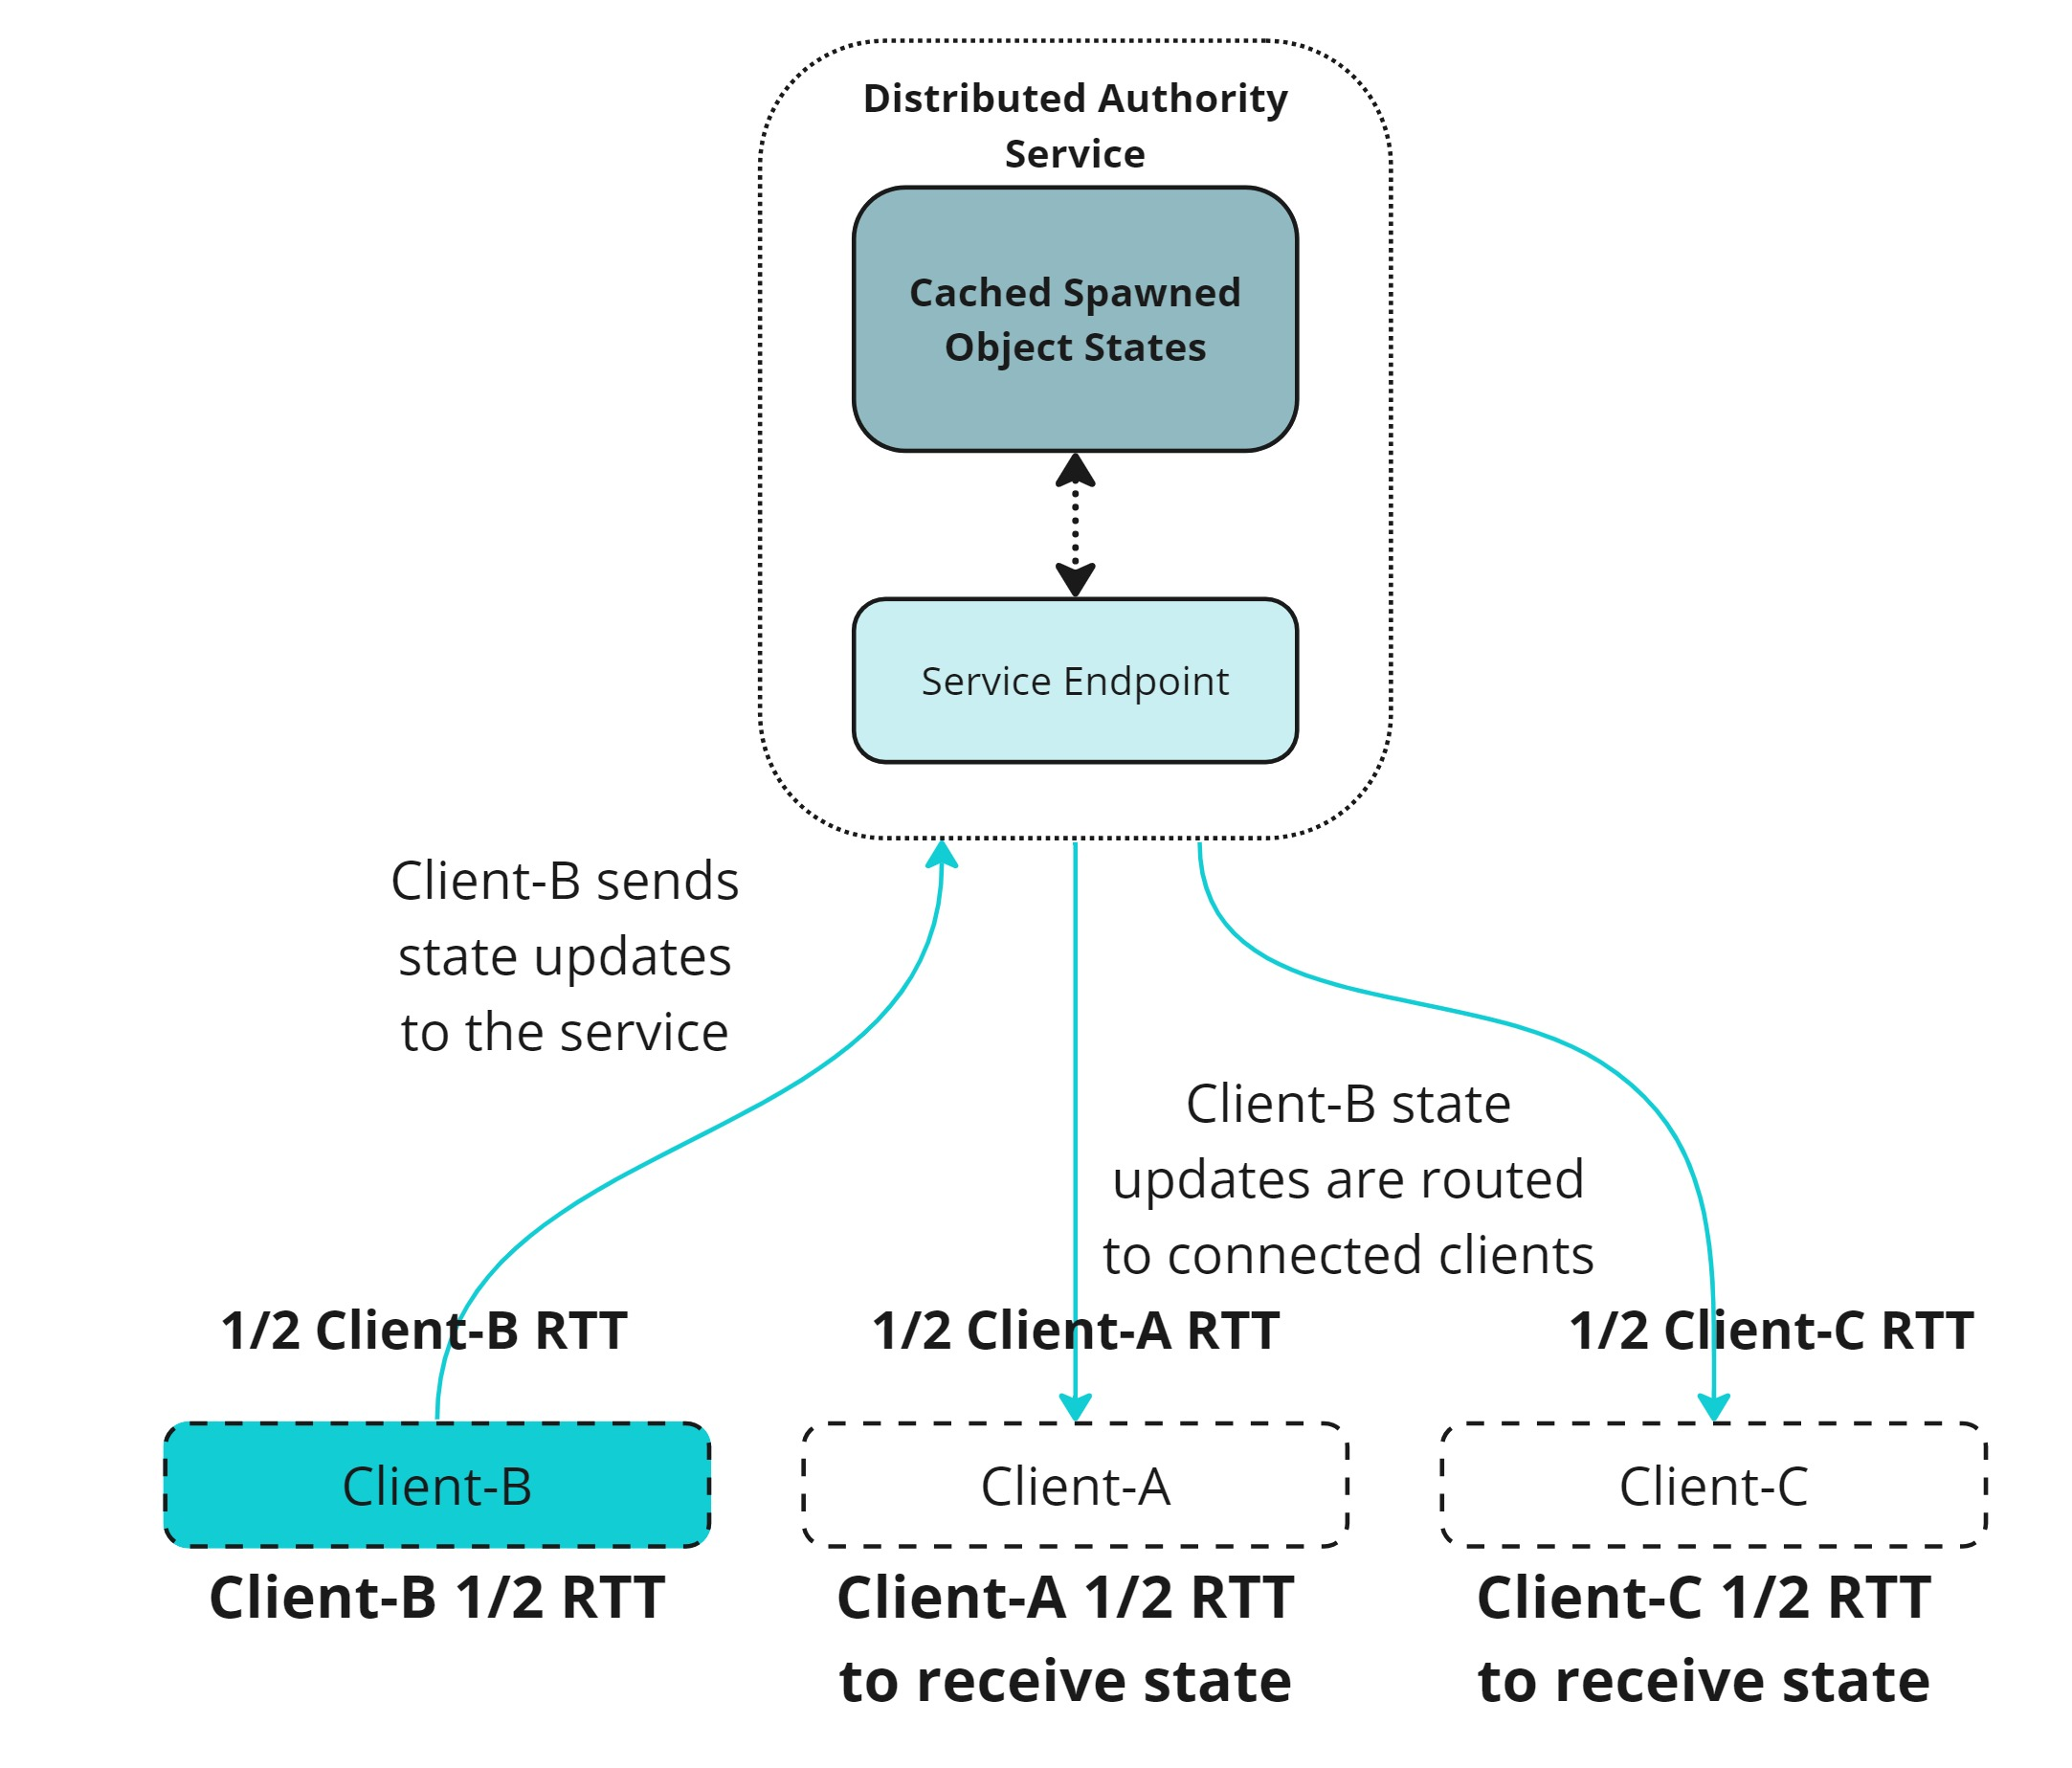
\includegraphics[width=1\linewidth]{content/pictures/distributed-authority-service.jpg}
\caption{Netzwerktopologie der Distributed Authority (Quelle: \citealp{noauthor_distributed_2025})}
\label{fig:distributed_authority_topology}
\end{figure}

Spiele wie \say{Journey}, \say{God of War: Ascension}, \say{Mercenaries 2}, \say{GTA: Online}, \say{Dark Souls} und \say{Destiny} nutzen diese Netzwerkinfrastruktur. Häufig kommt diese Topologie zum Einsatz, wenn ein bestehendes Singleplayer Spiel um eine Multiplayer-Komponente erweitert werden soll (Journey, GTA und Dark Souls), ohne den Kern des Quellcodes grundlegend umzustrukturieren. Diese Architektur erfordert keinen dedizierten Server. Sie eignet sich für Spiele mit großen, offenen Spielwelten (Dark Souls, GTA) und kommt häufig zum Einsatz, wenn keine deterministische Physik benötigt wird bzw. kein vollständigs deterministisches Spielkonzept vorliegt. Sie eignet sich zudem besonders für Spiele, bei denen die Prozessorleistung (z.B. durch Physiksimulationen) stark beansprucht wird. Für Spiele mit kooperativen Spielmechaniken, leichten kompetitiven Elementen oder innovativen Multiplayer-Ideen ist diese Infrastruktur eine sinnvolle Wahl (vgl. \citealp{noauthor_choosing_2024}).

\subsection{Pure Client/Server}
Bei der Client-Server-Architektur übernimmt ein zentraler Server die Hauptsimulation und verwaltet alle wesentlichen Aspekte des Spiels. Dazu gehören unter anderem die Physiksimulation, das Erzeugen und Entfernen von Objekten sowie die Autorisierung von Anfragen der Clients. Aus Sicht der Clients besitzen diese lediglich die Anwendung, über die sie sich mit dem Server verbinden. Sie erhalten über diese Verbindung die Darstellung des Spiels (vgl. \citealp{noauthor_client-server_2024}):
\paragraph{Ein dedizierter Server} bildet eine eigenständige Instanz, die ausschließlich dem Spielbetrieb dient (vgl. Abbildung \ref{fig:dedicated_server}).

\begin{figure}[ht]
\centering
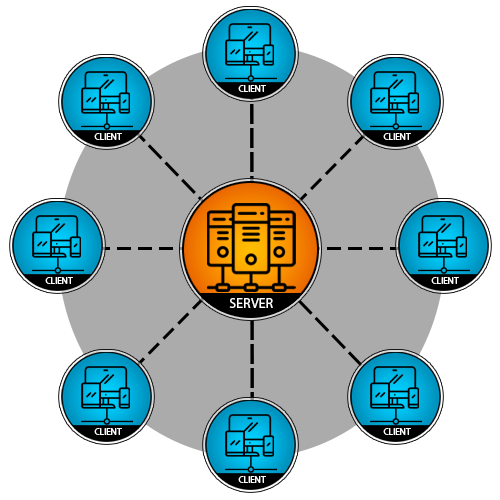
\includegraphics[width=1\linewidth]{content/pictures/ded_server-d5369721966357b9b4d5e1fa96b05b22.png}
\caption{Client-Server-Architektur mit dediziertem Server (Quelle: \citealp{noauthor_network_2024})}
\label{fig:dedicated_server}
\end{figure}

\paragraph{Ein Client gehosteter Server} läuft auf demselben Gerät wie die dazugehörige Client-Anwendung (vgl. Abbildung \ref{fig:client_server}).

\begin{figure}[ht]
\centering
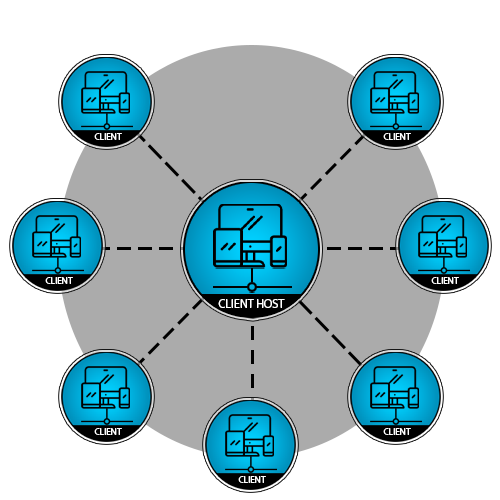
\includegraphics[width=1\linewidth]{content/pictures/client-hosted-16be0b1c9b5020f21325b1e6a7beca73.png}
\caption{Client hosted Server (Quelle: \citealp{noauthor_network_2024})}
\label{fig:client_server}
\end{figure}

\subsection{Peer-to-Peer}
Das \ac{P2P}-Architektur-Modell verbindet jeden Spieler direkt mit allen anderen. Über diese Verbindungen werden Daten zu Spielzuständen und Ereignissen ausgetauscht. Im \say{reinen} \ac{P2P}-System gibt es keinen zentralen \say{Host}. Stattdessen ist jeder Client dafür verantwortlich, seinen eigenen Avatar (oder seine Einheiten) zu verwalten und erhält gleichzeitig Updates von den anderen Clients (vgl. \citealp{mygames_unity_2024}). Abbildung \ref{fig:p-2-p} zeigt die entsprechende Topologie.

\begin{figure}[ht]
\centering
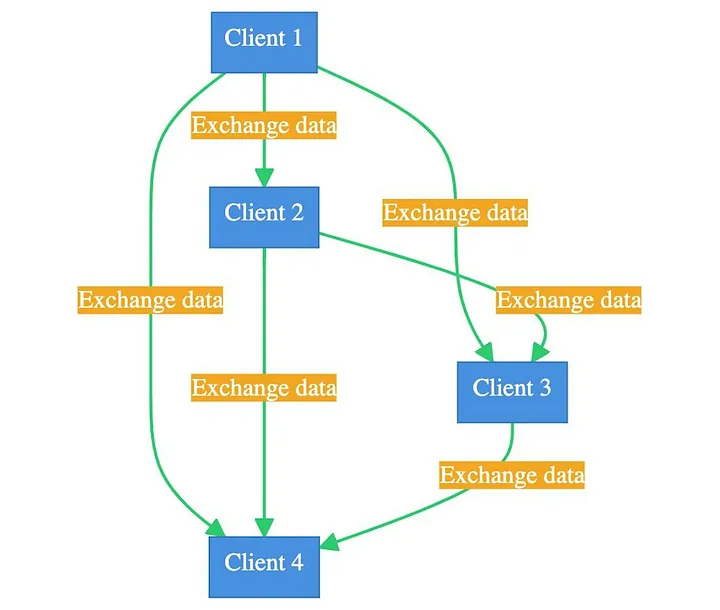
\includegraphics[width=1\linewidth]{content/pictures/0_poGQC2fWQ3tPWPwT.png}
\caption{Peer-to-Peer Infrastruktur (Quelle: \citealp{mygames_unity_2024})}
\label{fig:p-2-p}
\end{figure}


\subsection{Relay-Server}
Der Relay-Dienst ermöglicht Multiplayer-Unterstützung ohne die Notwenigkeit eines dedizierten Spielserver. Dabei wird die Kommunikation zwischen den Spielern über sogenannte Relay-Server weitergeleitet. Nachrichten werden mithilfe einer latenzarmen Datagramm-Übertragung übermittelt, sodass keine direkte Verbindung zwischen den einzelnen Spielern erforderlich ist (vgl. \citealp{noauthor_relay_nodate}).

\begin{figure}[ht]
\centering
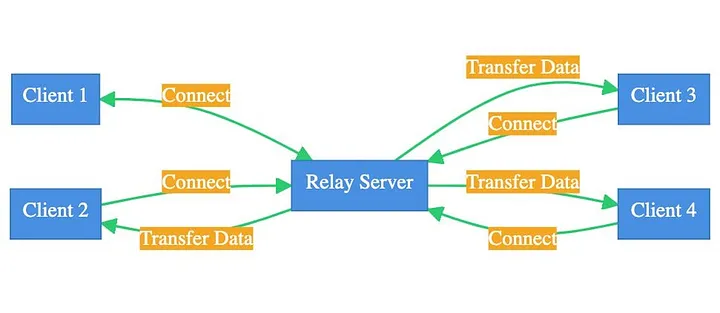
\includegraphics[width=1\linewidth]{content/pictures/0_o7LJU1ImxPHIM5Ej.png}
\caption{Relay-Server Infrastruktur (Quelle: \citealp{mygames_unity_2024})}
\label{fig:relay-server}
\end{figure}

\section{Augmented Reality}
Im Kontext der vorliegenden Arbeit stellt \ac{AR} eine essenzielle Technologie dar. Da eine der Anwendungen dieser Arbeit als \ac{AR}-Applikation konzipiert ist, ist es notwendig, grundlegende Definitionen, Abgrenzungen sowie technologische Grundlagen darzustellen. Im folgenden werden deshalb wesentliche theoretische und technische Aspekte erläutert, um das Verständnis für die im Spiel implementierten Interaktions- und Darstellungsmöglichkeiten zu gewährleisten.

\ac{AR} stellt eine Form virtueller Umgebungen (\ac{VE}) dar, bei der im Gegensatz zur vollständigen Immersion in rein virtuelle Welten, wie es in \ac{VR} der Fall ist, die Umgebung weiterhin sichtbar bleibt. Virtuelle Objekte werden dabei über die physische Welt gelegt und mit ihr kombiniert, sodass eine erweiterte Wahrnehmung entsteht. Es gewährleistet außerdem eine Interaktion mit den räumlich (\ac{3D}) registrierten virtuellen Inhalten in Echtzeit. Die technische Umsetzung kann dabei über monitorbasierte Schnittstellen, monokulare Systeme oder durchsichtige \ac{HMD}s erfolgen (vgl. \cite[S. 2f]{azuma_survey_1997}).

Im Vergleich zur \ac{VR}, das eine voll-immersive Umgebung erstellt, erweitert die \ac{AR} die eigene Realität und bietet dadurch die Möglichkeit, dass sich die Nutzer frei in der Welt bewegen können und auch immer noch mit der echten Welt interagieren können (vgl. \citealp[S. 79]{billinghurst_survey_2015}; \citealp[S. 1]{stefanidi_meaningful_2024}).

\subsection{Abgrenzung der Begriffe}
Sowohl in der Vergangenheit als auch in der aktuellen Forschung werden intensiv Konzepte und Ansätze zur Integration und Verbesserung von \ac{AR} und \ac{VR} untersucht. Damit zwischen diesen Begriffen und den weiteren in der Forschung angewandten Begriffen \ac{MR} oder \ac{XR} unterschieden werden kann, wurde von  \cite{milgram_taxonomy_1994} das Konzept des \say{\ac{VC}s} entworfen (vgl. Abbildung \ref{fig:virtuality-continuum}).

\begin{figure}[ht]
\centering
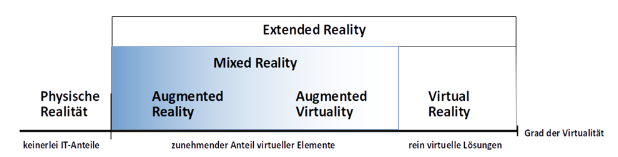
\includegraphics[width=1\linewidth]{content/pictures/virtuality-continuum_upscaled.PNG}
\caption{Vereinfachte Darstellung eines "Virtuality Continuums" (Quelle: \citealp[S. 9]{knoll_augmented_2022}; Modifiziert nach \citealp[S. 3]{milgram_taxonomy_1994})}
\label{fig:virtuality-continuum}
\end{figure}

Auf der linken Seite des \ac{VC}s befindet sich die reale Umgebung (\ac{PR}), während auf der gegenüberliegenden rechten Seite die vollständig virtuellen Umgebung (\ac{VR}) verortet ist. Je weiter sich innerhalb des Kontinuums von der virtuellen hin zur realen Seite bewegt wird, desto stärker tritt die physische Welt in den Vordergrund, wobei virtuelle Elemente zunehmend überlagert und mit realen Inhalten kombiniert werden. 
Die \ac{PR} umfasst ausschließlich reale Objekte und Umgebungen ohne virtuelle Erweiterungen. \ac{AR} beschreibt einen Zwischenbereich, in dem digitale Inhalte on die reale Welt eingeblendet und mit dieser in Echtzeit kombiniert werden. Im der \ac{AV} hingegen befindet sich der Nutzer in einer primär virtuellen Umgebung, die durch ausgewählte Elemente aus der realen Welt ergänzt wird. Die \ac{VR} bildet schließlich das andere Extrem des Spektrums, bei dem sich der Nutzer in einer vollständig künstlich erzeugten Umgebung aufhält und mit dieser interagiert (vgl. \citealp[S. 3]{milgram_taxonomy_1994}; \citealp[S. 8f]{knoll_augmented_2022}; \citealp[S. 3]{zuniga_gonzalez_making_2021}).

Der Begriff der \ac{XR} dient als Oberkategorie für sämtliche Ausprägungen von Technologien, bei denen virtuelle Inhalte zur Erweiterung oder Ersetzung der realen Umgebung zum Einsatz kommen. Dazu zählen insbesondere \ac{AR}, \ac{AV} und \ac{VR}. Innerhalb dieses Spektrums bezeichnet \ac{MR} diejenigen Anwendungen, in denen reale und virtuelle Inhalte nicht nur koexistieren, sondern in Echtzeit miteinander interagieren. Diese schließt sowohl Szenarien ein, in denen virtuelle Objekte die physische Welt überlagern, als auch solche, in denen reale Elemente in einer primär virtuellen Umgebung integriert werden (vgl. Abbildung \ref{fig:virtuality-continuum}).

\subsection{Technologische Umsetzungen}
Die Integration der virtuellen Elemente in die physische Umgebung kann mithilfe verschiedener Ansätze realisiert werden. Zu den am weitesten verbreiteten Ausgabetechnologien zählen mobile Endgeräte wie Smartphones und Tablets, \ac{HMD}s sowie projektionsbasierte Systeme. Im folgenden werden diese unterschiedlichen Technologien vorgestellt.
\begin{figure}[ht]
\centering
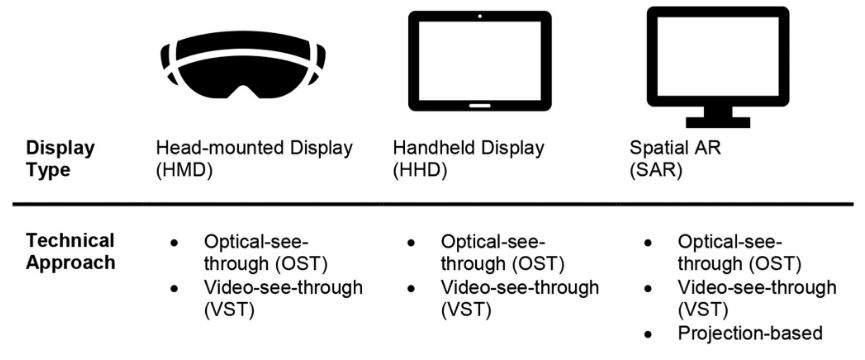
\includegraphics[width=1\linewidth]{content/pictures/devices.PNG}
\caption{Klassifizierungen von Augmented Reality Displays (Quelle: \citealp[S. 315]{leins_comparing_2024})}
\label{fig:ar-classes}
\end{figure}

\paragraph{\ac{HAR}}

\begin{figure}[ht]
\centering
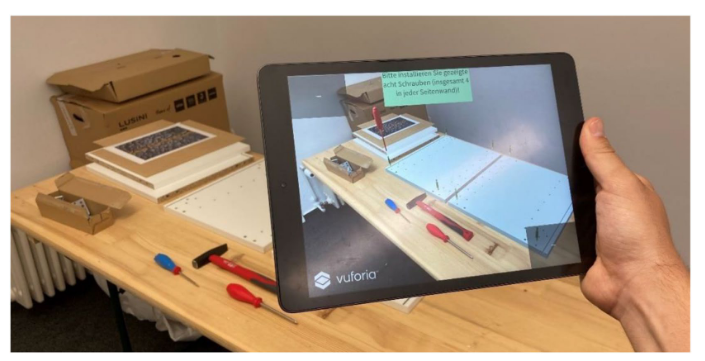
\includegraphics[width=0.5\linewidth]{content/pictures/handheld-ar.PNG}
\caption{Handheld-AR Display (Quelle: \citealp[S. 318]{leins_comparing_2024})}
\label{fig:handheld-ar}
\end{figure}

bezeichnet die Verwendung tragbarer Endgeräte, wie Smartphones oder Tablets, zur Darstellung erweiterter Realitäten. Diese GEräte werden in der Hand gehalten und nutzen typischerweise Video-see-through-Technologien, bei denen die reale Umgebung über die Kameralinse erfasst und auf dem Display mit virtuellen Inhalten überlagert dargestellt wird (vgl. Abbildung \ref{fig:handheld-ar}). Zur präzisen Bestimmung von Position und Ausrichtung der Kamera greifen \ac{HAR}-Systeme auf eine Kombination integrierter Sensoren zurück. Digitale Kompasse, GPS-Module, Gyroskope und Beschleunigungssensoren ermöglichen eine räumlich korrekte Platzierung virtueller Objekte in Echtzeit und unterstützen eine dynamische Interaktion mit der Umgebung (vgl. \citealp[S. 347]{carmigniani_augmented_2011}).

\paragraph{\ac{HMD}}

\begin{figure}[ht]
\centering
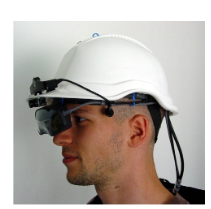
\includegraphics[width=0.5\linewidth]{content/pictures/hmd-ar.PNG}
\caption{Head-Mounted-Display (Quelle: \citealp[S. 4]{reitmayr_location_2003})}
\label{fig:hmd-ar}
\end{figure}

sind tragbare Anzeigesysteme, die direkt am Kopf oder als Bestandteil eines Helms getragen werden und es ermöglichen, sowohl reale als auch virtuelle Inhalte simultan im Sichtfeld des Nutzers darzustellen (vgl. Abbildung \ref{fig:hmd-ar}). Diese Geräte können verschiedene technologische Ansätze zur Überlagerung visueller Informationen verwenden, insbesondere Video-see-through- und optische see-through-Technologien, jeweils in mono- oder binokularer Ausführung (vgl. \citealp[S. 346]{carmigniani_augmented_2011}).

Bei Video-see-through-Systemen wird die reale Umgehung durch am \ac{HMD} montierte Kameras erfasst, deren Bilddaten in Echtzeit mit den virtuellen Inhalten verrechnet und auf dem Display ausgegeben werden. Da hierbei eine kontinuierliche Bildverarbeitung erforderlich ist, sind solche Systeme mit einem hohen Rechen aufwand verbunden. Ein aktuelles Beispiel für ein solches System die die \cite{htc_vive_2023}). Im Gegensatz dazu ermöglichen optische see-through-Systeme die direkte Sicht auf die physische Umgebung, indem sie halbtransparente Spiegel oder Displays (eine sog. Halbspiegeltechnologie) nutzen, die virtuelle Inhalte über das reale Sichtfeld projizieren. Diese Technologie erfordert vergleichsweise weniger Rechenleistung, da keine vollständige Kamerabildverarbeitung notwendig ist (vgl. \citealp[S. 346f]{carmigniani_augmented_2011}).

\paragraph{\ac{SAR}}
\begin{figure}[ht]
\centering
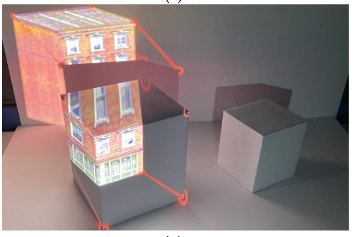
\includegraphics[width=0.5\linewidth]{content/pictures/spatial-ar.PNG}
\caption{Spatial Augmented Reality (Quelle: \citealp[S. 7]{jin_bim-based_2020})}
\label{fig:spatial-ar}
\end{figure}

Bei \ac{SAR} werden grafische Informationen mithilfe von Videoprojektoren und weiteren Tracking-Technologien direkt auf die physische Objekte in der realen Umgebung projiziert (vgl. Abbildung \ref{fig:spatial-ar}). Im gegensatz zu den anderen \ac{AR}-Systemen ist bei \ac{SAR} nicht erforderlich, dass Nutzer ein Display tragen oder ein Gerät in der Hand halten. Die Technologie wird stattdessen größtenteils in die Umgebung integriert, wodurch eine natürliche und geräteunabhängige Interaktion mit virtuellen Inhalten ermöglicht wird (vgl. \citealp[S. 348]{carmigniani_augmented_2011}).

Grundsätzlich lassen sich drei technische Ansätze innerhalb der \ac{SAR} unterscheiden. Bildschirmbasierte Video-see-through-Systeme verwenden kostengünstige, handelsübliche Hardwarekomponenten und ermöglichen die Darstellung erweiterter Inhalte über stationäre Bildschirme. Aufgrund ihrer geringen Mobilität sind sie jedoch auf fest installierte Anwendungen beschränkt. Räumliche optische see-through-Systeme hingegen nutzen optische Komponenten wie Spiegelstrahler oder transparente Projektionsflächen, um digitale Inhalte direkt im Raum visuell zu verankern. Auch sie sind nicht für mobile Nutzung konzipiert, bieten jedoch eine realitätsnahe Integration virtueller Informationen. Projektorbasierte \ac{SAR}-Systeme projizieren Bilder unmittelbar auf reale Oberflächen und erlauben somit eine besondere immersive Verschmelzung zwischen physischer und virtueller Umgebung (vgl. \citealp[S. 348]{carmigniani_augmented_2011}).

\subsection{Platzierungsmethoden virtueller Objekte}
Damit virtuelle Objekte in \ac{AR}-Anwendungen sinnvoll in die physische Umgebung integriert werden können, ist eine präzise räumliche Platzierung dieser Inhalte erforderlich. Zu diesem Zweck existieren unterschiedliche Platzierungsmethoden, die je nach technologischem Ansatz, Anwendungskontext und verfügbaren Sensoren variieren. Abbildung \ref{fig:placement-ar} gibt einen Überblick über Verfahren zur Positionierung virtueller Inhalte in \ac{AR}-Systemen.

\begin{figure}[ht]
\centering
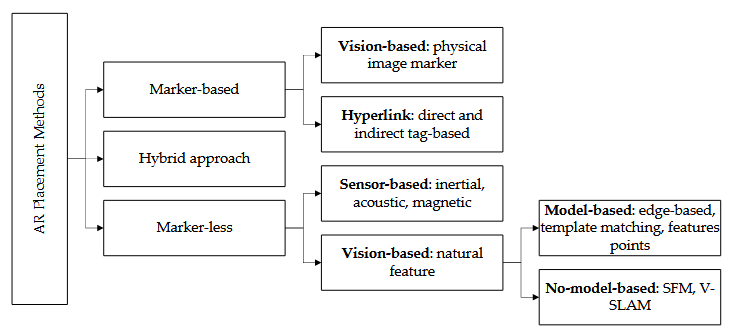
\includegraphics[width=1\linewidth]{content/pictures/placement-methods.PNG}
\caption{Verschiedene Platzierungsmethoden in Augmented Reality (Quelle: \citealp[S. 3]{el_barhoumi_assessment_2022})}
\label{fig:placement-ar}
\end{figure}

Eine der gebräuchlichsten Methoden zur Platzierung virtueller Inhalte in \ac{AR}-Systemen stellt der markerbasierte Ansatz dar. 
Dabei werden virtuelle Objekte anhand spezifischer Marker in der physischen Umgebung positioniert. Grundsätzlich lassen sich zwischen Hyperlink- und kamerabasierte Methoden unterscheiden. Erstere verknüpfen physische Objekte über grafische Tags oder automatische Identifikationstechnologien mit webbasierten Inhalten. Kamerabasierte Verfahren hingegen erkennen gedruckte Muster oder reale Objekte durch Analyse des Kamerabildes, um daran orientiert virtuelle Inhalte zu plattieren (vgl. \citealp[S. 3f]{el_barhoumi_assessment_2022}). 

Demgegenüber stehen markerlose Verfahren, die sich in sensorbasierte und kamerabasierte Ansätze untergliedern lassen. Sensorbasierte Methoden nutze die in den mobilen Endgeräten integrieren Sensoren um Position und Orientierung der Kamera zu bestimmen. Kamerabasierte Verfahren lassen sich weiter differenzieren in modellbasierte und nicht-modellbasierte Ansätze. Modellbasierte Techniken setzen meist ein vorhandenes \ac{3D}-Modell der Umgebung voraus. Über kanten- und merkmalbasiertes Tracking werden Merkmale aus dem Kamerabild mit dem Modell abgeglichen. Auch Verfahren des Template-Matching, bei dem kleinere Bildausschnitte mit Datenbankeinträgen verglichen werden, sowie Methoden, die Tiefeninformationen zur räumlichen Erfassung nutzen, kommen in diesem Zusammenhang zum Einsatz. Nicht-modellbasierte Ansätze hingegen benötigen kein vorab erstelltes Modell. Stattdessen rekonstruieren sie die Umgebung simultan während der Kamerabewegung (vgl. \citealp[S. 4f]{el_barhoumi_assessment_2022}).

Hybride \ac{AR}-Ansätze kombinieren die vorangegangenen Methoden, um deren jeweilige Nachteile zu kompensieren. Sie ermöglichen präzisiere und robustere Anwendungen bei geringerer Rechenlast (vgl. \citealp[S. 5]{el_barhoumi_assessment_2022}.